\documentclass[10pt]{article}
\usepackage[margin=1in]{geometry}
\usepackage[utf8]{inputenc}
\usepackage{multicol}
\setlength{\columnsep}{1mm}
\usepackage{amsfonts}
\usepackage{booktabs}
\usepackage{siunitx}
\usepackage[authoryear,round]{natbib}
\usepackage{float}
\usepackage[font={small}]{caption}
\usepackage[labelfont=bf]{caption}
\usepackage{lineno}
\usepackage{amsmath,amssymb,setspace,fancyhdr,geometry,url,color}
\usepackage{subfigure,graphicx,caption}
\usepackage{lscape,amsthm}
\usepackage{blindtext}
\usepackage{hhline}
\usepackage{arydshln}
\usepackage{verbatim}
\usepackage{dblfloatfix}
\usepackage{multirow}
\usepackage{graphicx}
\usepackage{xr}

\externaldocument{../PhaseIIPaper/Part1/main1}

\renewcommand\thefigure{S\arabic{figure}}
\renewcommand\thetable{S\arabic{table}}
\renewcommand\thesection{S\arabic{section}}
\setcounter{table}{0}
\setcounter{figure}{0}

%\biboptions{authoryear, comma}
%%%%%%%%%%%%%%%%%%%%%%%%%%%%%%%%%%%%%%%%%%%%%%%%%%%%%%%%%%%%%%%%%%%%%%%%%
%%%%%%%%%%%%%%%%%%%%%%%%%%%%%%%%%%%%%%%%%%%%%%%%%%%%%%%%%%%%%%%%%%%%%%%%%%
\begin{document}
\centering{\bf {\large Supplemental Material} \\
{\Large The GGCMI Phase II experiment: global gridded crop model simulations under uniform changes in CO$_2$, temperature, water, and nitrogen levels (protocol version 1.0)}}\\

\vspace{3mm}

\centering{James Franke$^{1, 2}$, 
Christoph M\"{u}ller$^3$, 
Joshua Elliott$^{2, 4}$, 
Alexander Ruane$^5$, 
Abigail Snyder$^6$,\\ 
Jonas J\"{a}germeyr$^{3, 2, 4, 5}$, 
Juraj Balkovic$^{7, 8}$, 
Philippe Ciais$^{9, 10}$, 
Marie Dury$^{11}$, 
Pete Falloon$^{12}$,\\ 
Christian Folberth$^7$, 
Louis Fran{\c{c}}ois$^{11}$, 
Tobias Hank$^{13}$, 
Munir Hoffmann$^{14,23}$, 
Cesar Izaurralde$^{15, 16}$,\\ 
Ingrid Jacquemin$^11$, 
Curtis Jones$^{15}$, 
Nikolay Khabarov$^7$, 
Marian Koch$^{14}$, 
Michelle Li$^{2, 17}$, 
Wenfeng Liu$^{18, 9}$,\\ 
Stefan Olin$^{19}$, 
Meridel Phillips$^{5, 20}$, 
Thomas Pugh$^{21, 22}$, 
Ashwan Reddy$^{15}$, 
Xuhui Wang$^{9, 10}$,\\ 
Karina Williams$^{12}$, 
Florian Zabel$^{13}$, 
and Elisabeth Moyer$^{1, 2}$\\
~\\}

\centering{
{\small 1.  Department of the Geophysical Sciences, University of Chicago, Chicago, IL, USA}\\
{\small 2.  Center for Robust Decision-making on Climate and Energy Policy, University of Chicago, Chicago, IL, USA}\\
{\small 3.  Potsdam Institute for Climate Impact Research, Leibniz Association (Member), Potsdam, Germany}\\
{\small 4.  Department of Computer Science, University of Chicago, Chicago, IL, USA}\\
{\small 5.  NASA Goddard Institute for Space Studies, New York, NY, United States}\\
{\small 6.  Joint Global Change Research Institute, Pacific Northwest National Laboratory, College Park, MD, USA}\\
{\small 7.  Ecosystem Services and Mgm. Prg., International Institute for Applied Systems Analysis, Laxenburg, Austria}\\
{\small 8.  Department of Soil Science, Comenius University in Bratislava, Bratislava, Slovak Republic}\\
{\small 9.  Laboratoire des Sciences du Climat et de l'Environnement,CEA-CNRS-UVSQ, 91191 Gif-sur-Yvette, France}\\
{\small 10. Sino-French Institute of Earth System Sciences, Peking University, Beijing, China}\\
{\small 11. Unit{\'{e}} de Mod{\'{e}}lisation du Climat et des Cycles Biog\'eochimiques, University of Li\`ege, Belgium}\\
{\small 12. Met Office Hadley Centre, Exeter, United Kingdom}\\
{\small 13. Department of Geography, Ludwig-Maximilians-Universit\"{a}t, Munich, Germany}\\
{\small 14. Georg-August-University G\"{o}ttingen, Tropical Plant Production and Ag. Sys. Modelling, G\"{o}ttingen, Germany}\\
{\small 15. Department of Geographical Sciences, University of Maryland, College Park, MD, USA}\\
{\small 16. Texas Agrilife Research and Extension, Texas A\&M University, Temple, TX, USA}\\
{\small 17. Department of Statistics, University of Chicago, Chicago, IL, USA}\\
{\small 18. EAWAG, Swiss Federal Institute of Aquatic Science and Technology, D\"{u}bendorf, Switzerland}\\
{\small 19. Department of Physical Geography and Ecosystem Science, Lund University, Lund, Sweden}\\
{\small 20. Earth Institute Center for Climate Systems Research, Columbia University, New York, NY, USA}\\
{\small 21. Karlsruhe Institute of Technology, IMK-IFU, 82467 Garmisch-Partenkirchen, Germany}\\
{\small 22. School of Geography, Earth and Environmental Science, University of Birmingham, Birmingham, UK}\\
{\small 23. Leibniz Centre for Agricultural Landscape Research (ZALF), D-15374 Müncheberg, Germany}
}

%\tableofcontents

%%%%%%%%%%%%%%%%%%%%%%%%%%%%%%%%%%%
\clearpage
%%%%%%%%%%%%%%%%%%%%%%%%%%%%%%%%%%%
\renewcommand{\thefigure}{S\arabic{figure}}

\section{Cultivation Areas}
\begin{figure}[h!]
\centering
%S1
\begin{minipage}{.45\textwidth}
    \centering
    \vspace{0pt}
    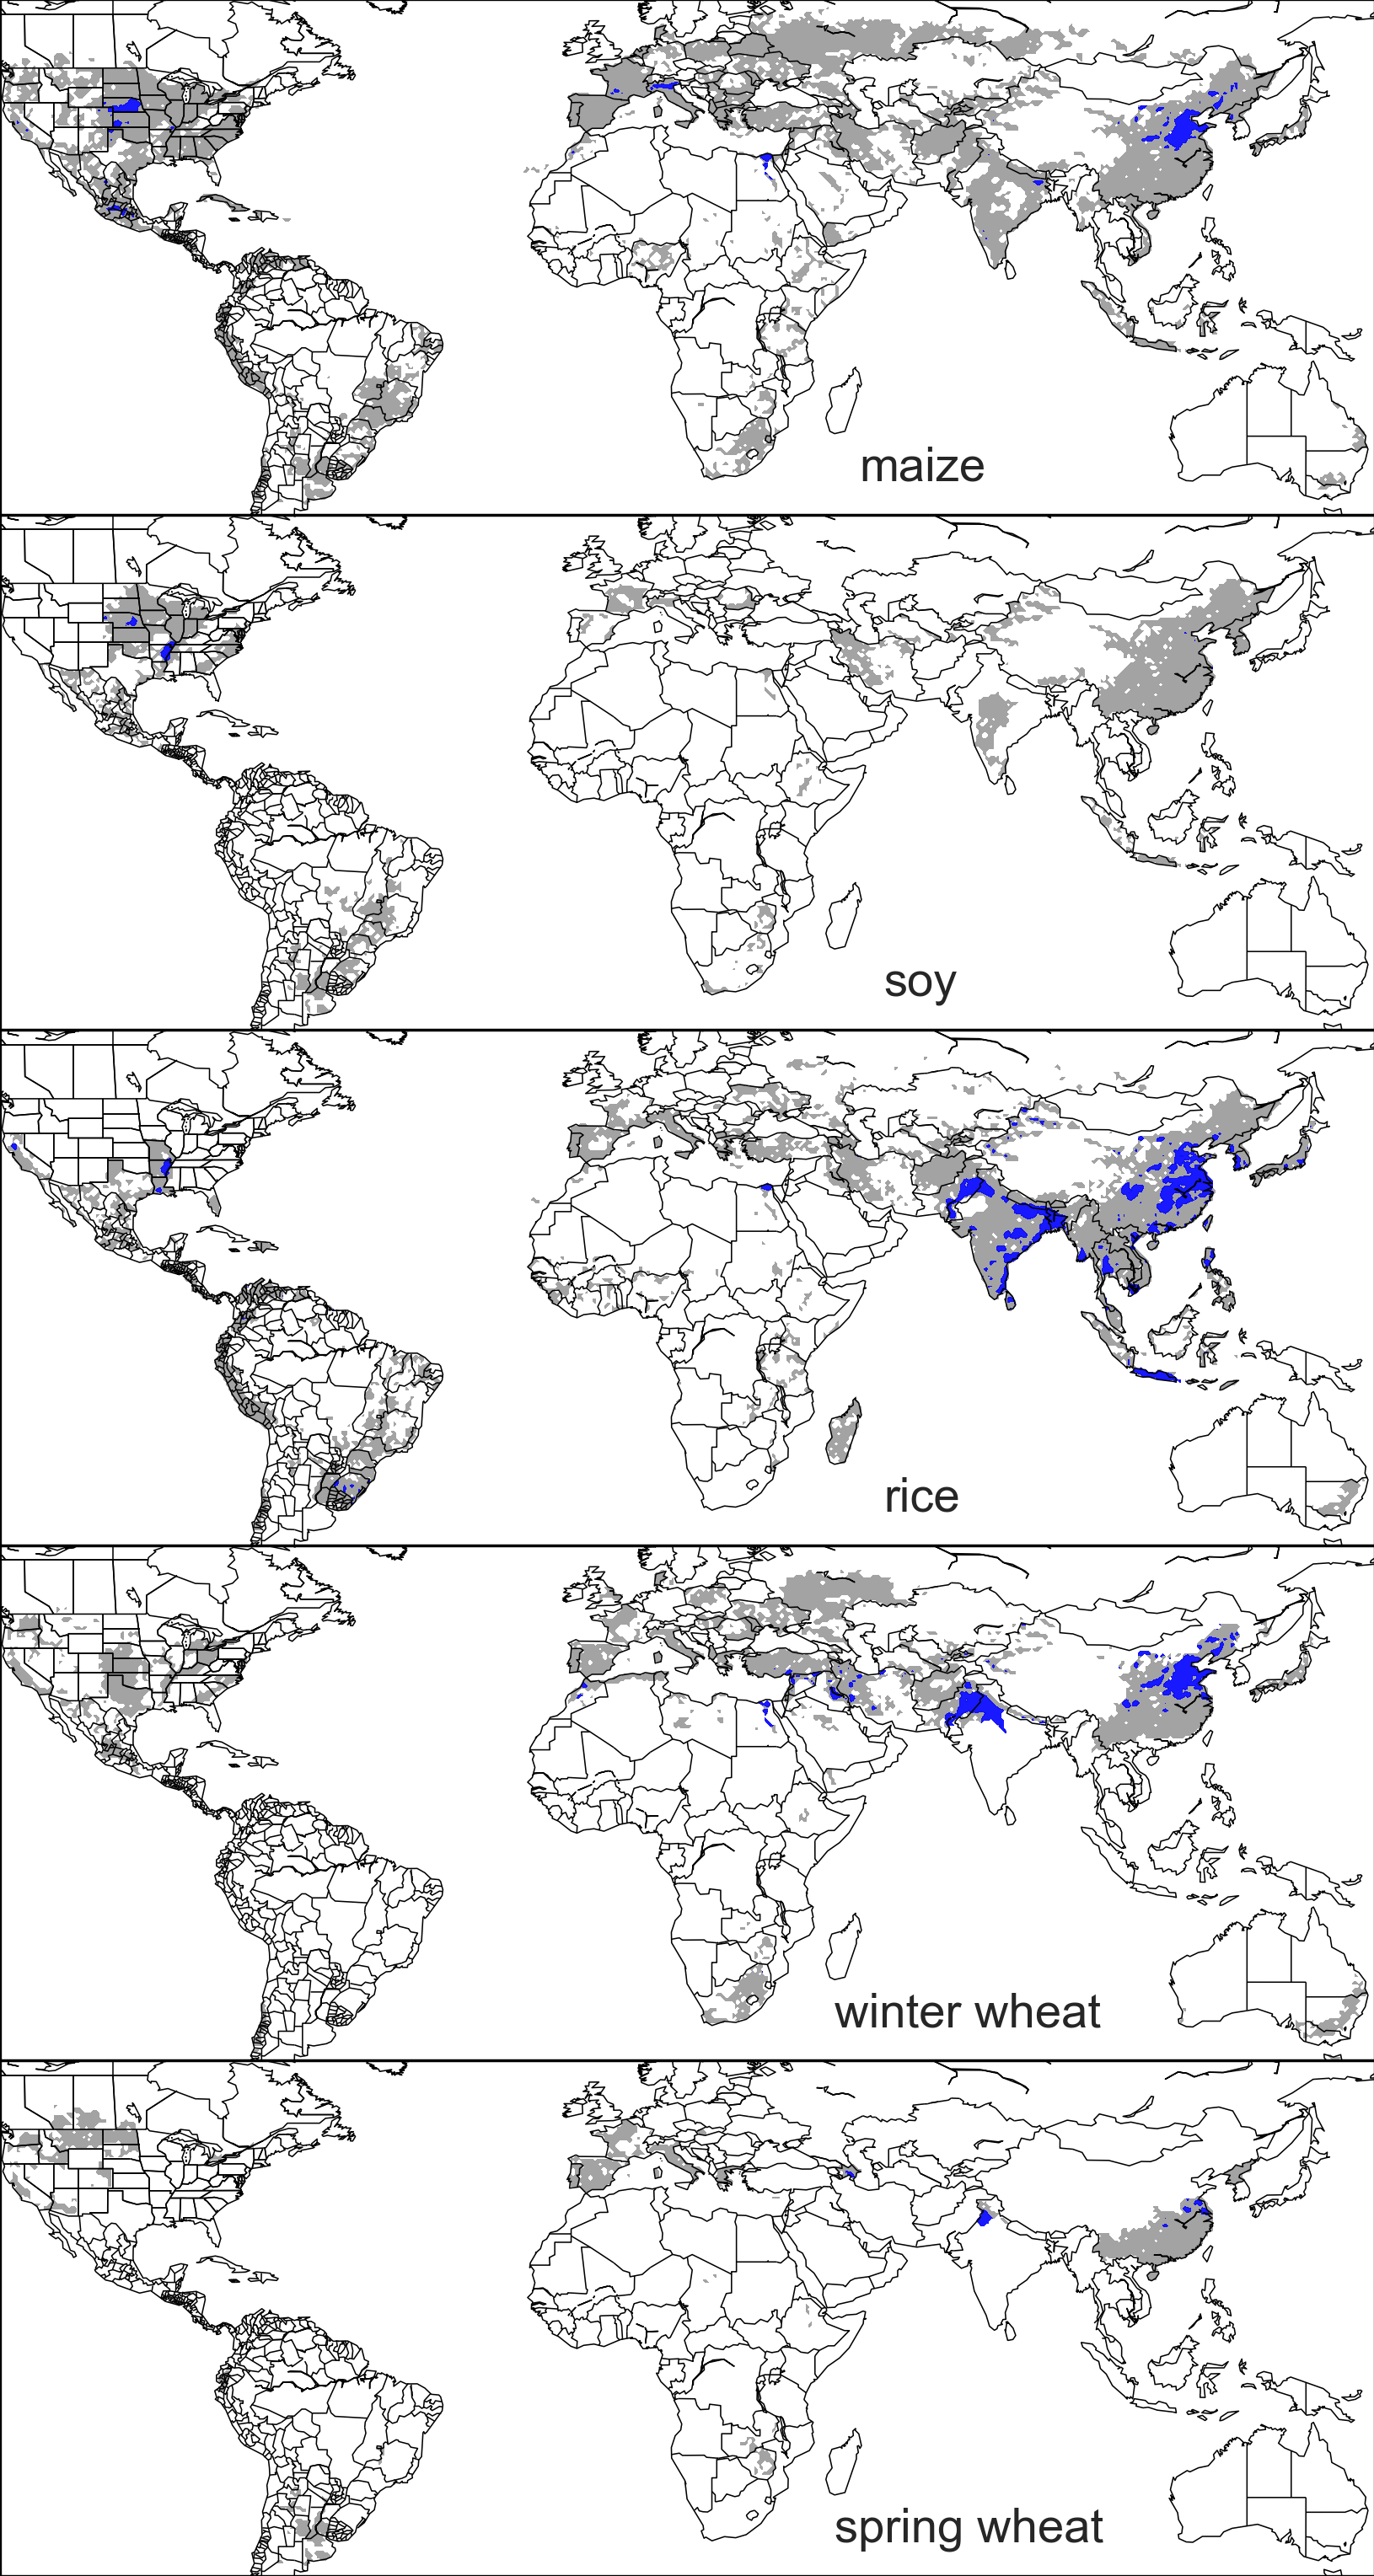
\includegraphics[width=\textwidth]{s_croparea_irr.png}\\
    \caption{Presently cultivated area for irrigated crops in the real world. The blue contour area indicates grid-cells with more that 20,00 hectares of crop cultivated. The gray contour shows area with more that 10 hectares cultivated. Data from the MIRCA2000 data set for maize, rice, and soy. Winter and spring wheat areas are adapted from MIRCA2000 data and sorted by growing season.}
    \label{fig:irrarea}
\end{minipage}
\hspace{.05\linewidth}
%S2
\begin{minipage}{.45\textwidth}
    \centering
    \vspace{-19mm}
    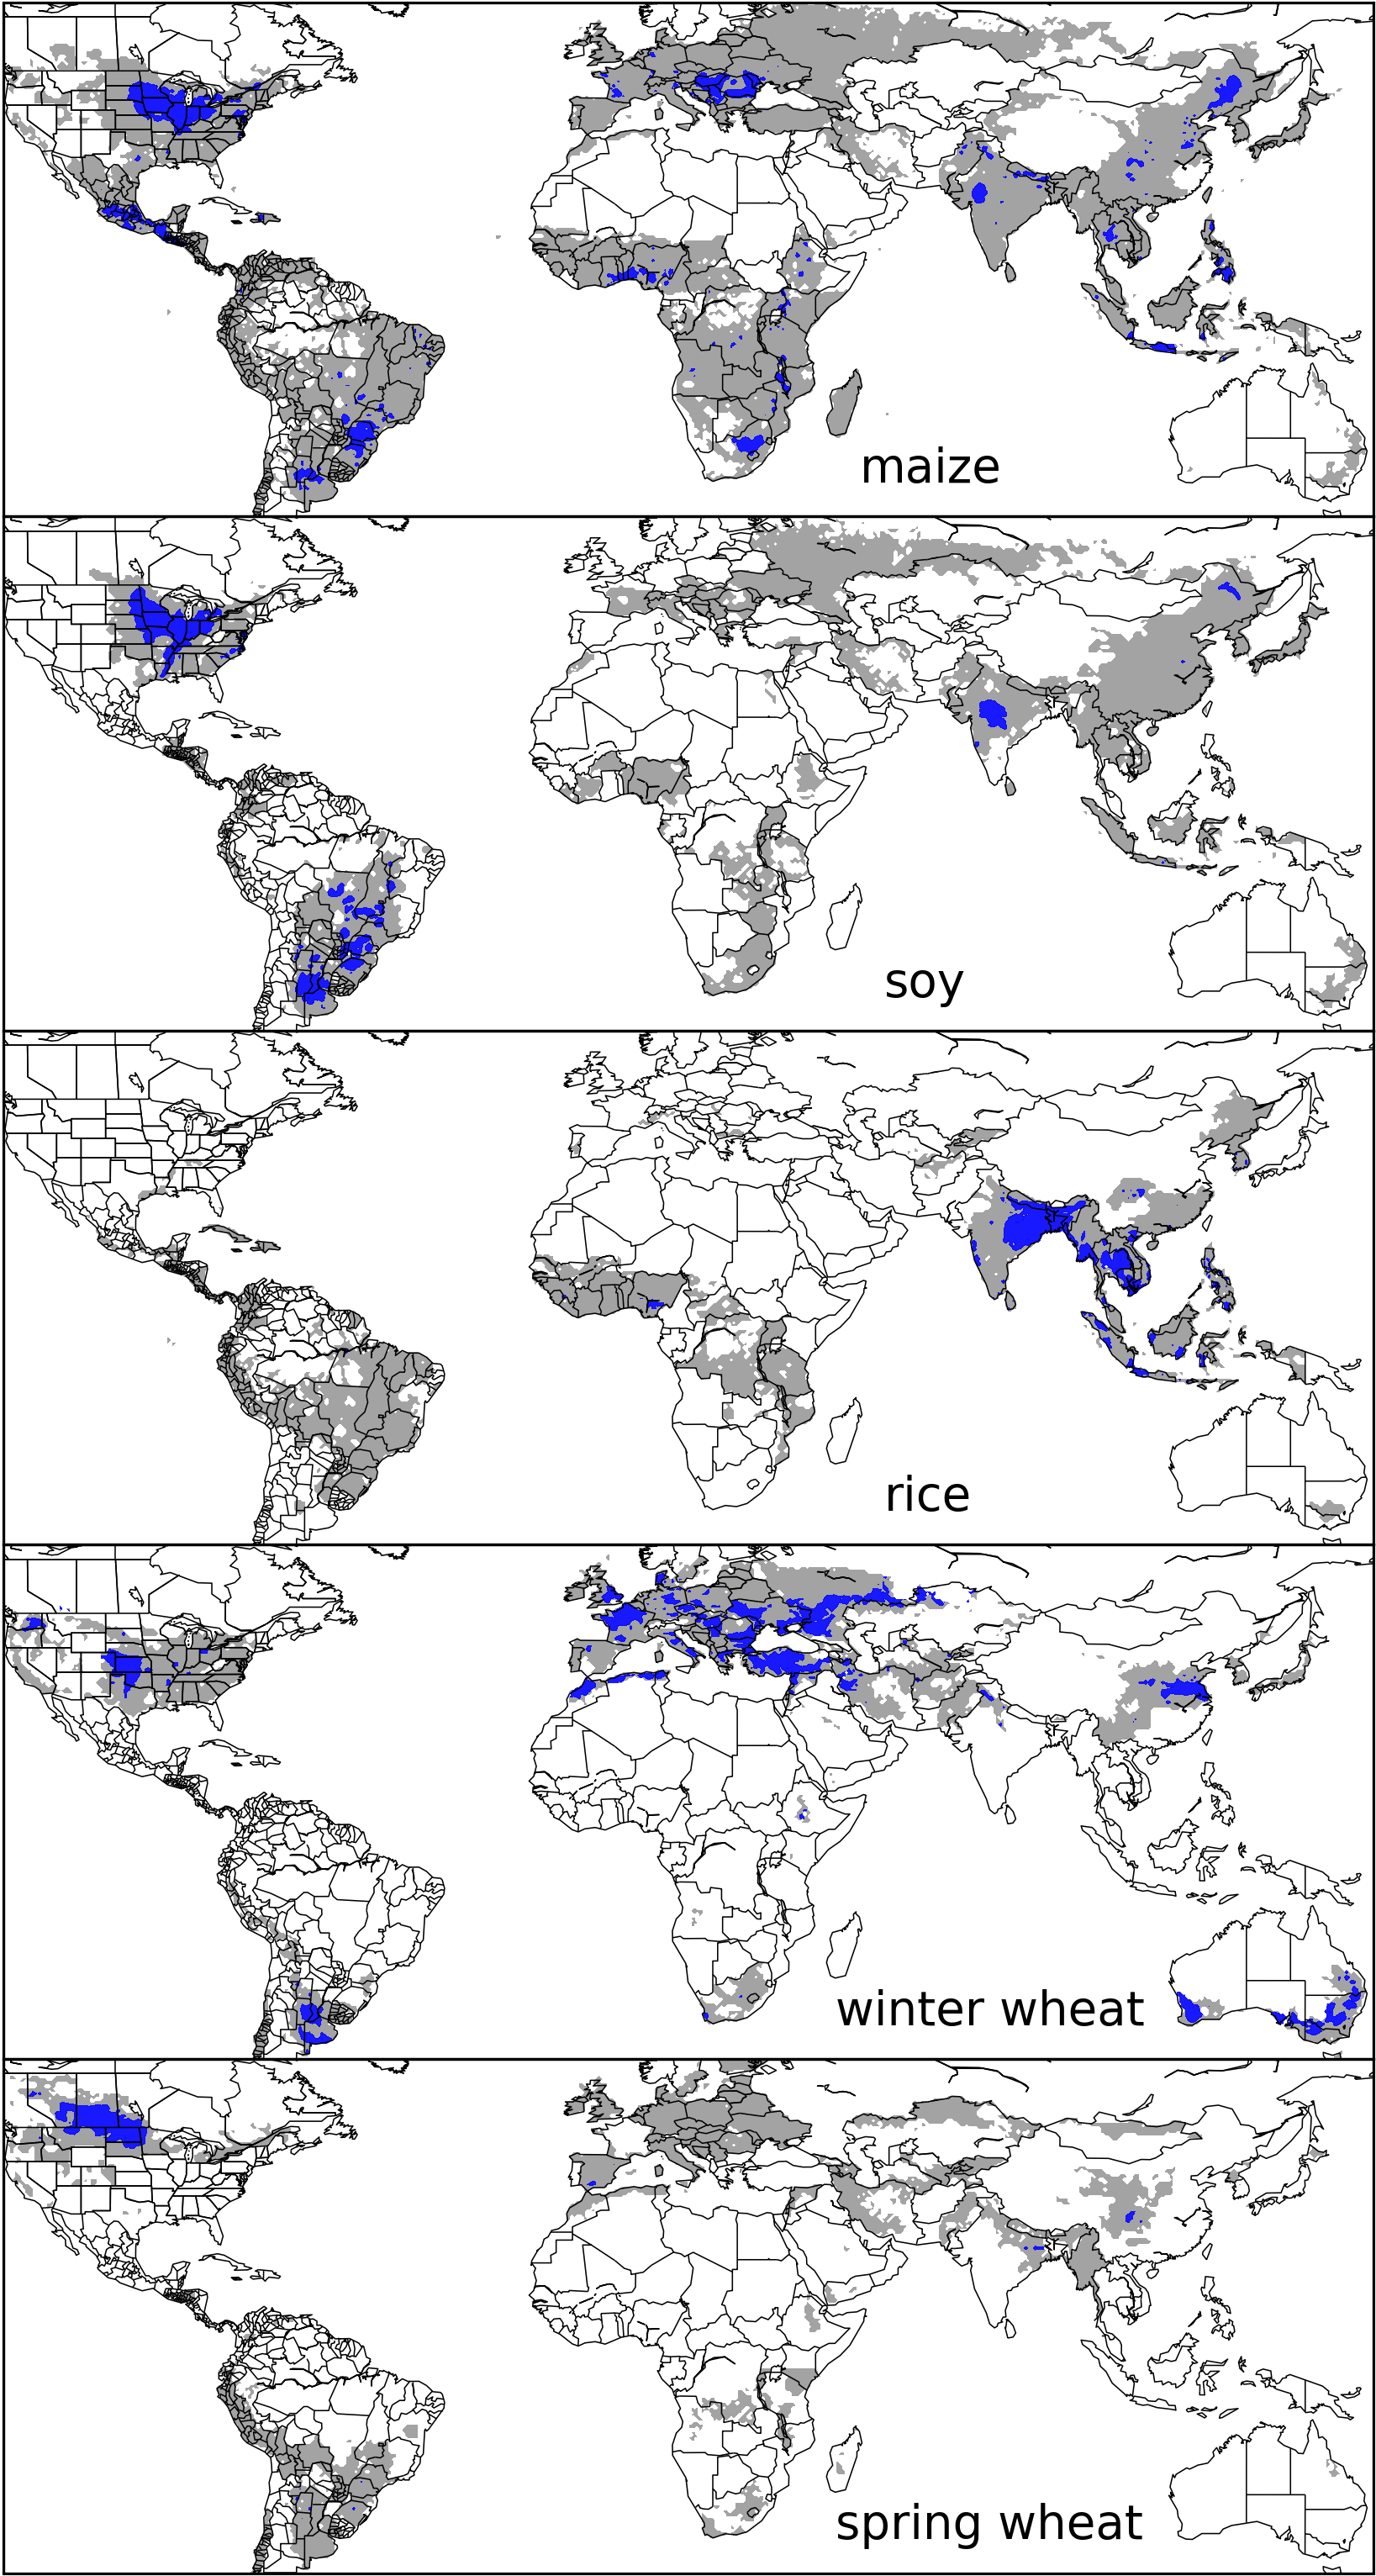
\includegraphics[width=\textwidth]{s_croparea.png}\\
    \caption{Presently cultivated area for rain fed crops in the real world. Conventions as in Figure S1. This figure repeats manuscript Figure 1 for ease of comparison.}
    \label{fig:rainfed}
\end{minipage}
\end{figure}

\clearpage
\section{Reanalysis Climate Products}
\begin{figure}[h!]
\centering
\includegraphics[width=\textwidth]{s_precip_rea.png}
\caption{Depreciation comparison across the three reanalysis products used in GGCMI Phase II. Values are aggregated across cultivation area based on the MIRCA2000 dataset.}
\label{fig:precip_rea}
\end{figure}

\begin{figure}[h!]
\centering
\includegraphics[width=\textwidth]{s_temp_rea.png}
\caption{Same as S3 but for temperature.}
\label{fig:precip_rea}
\end{figure}

\clearpage
\section{Results}
\begin{figure}[h!]
\centering
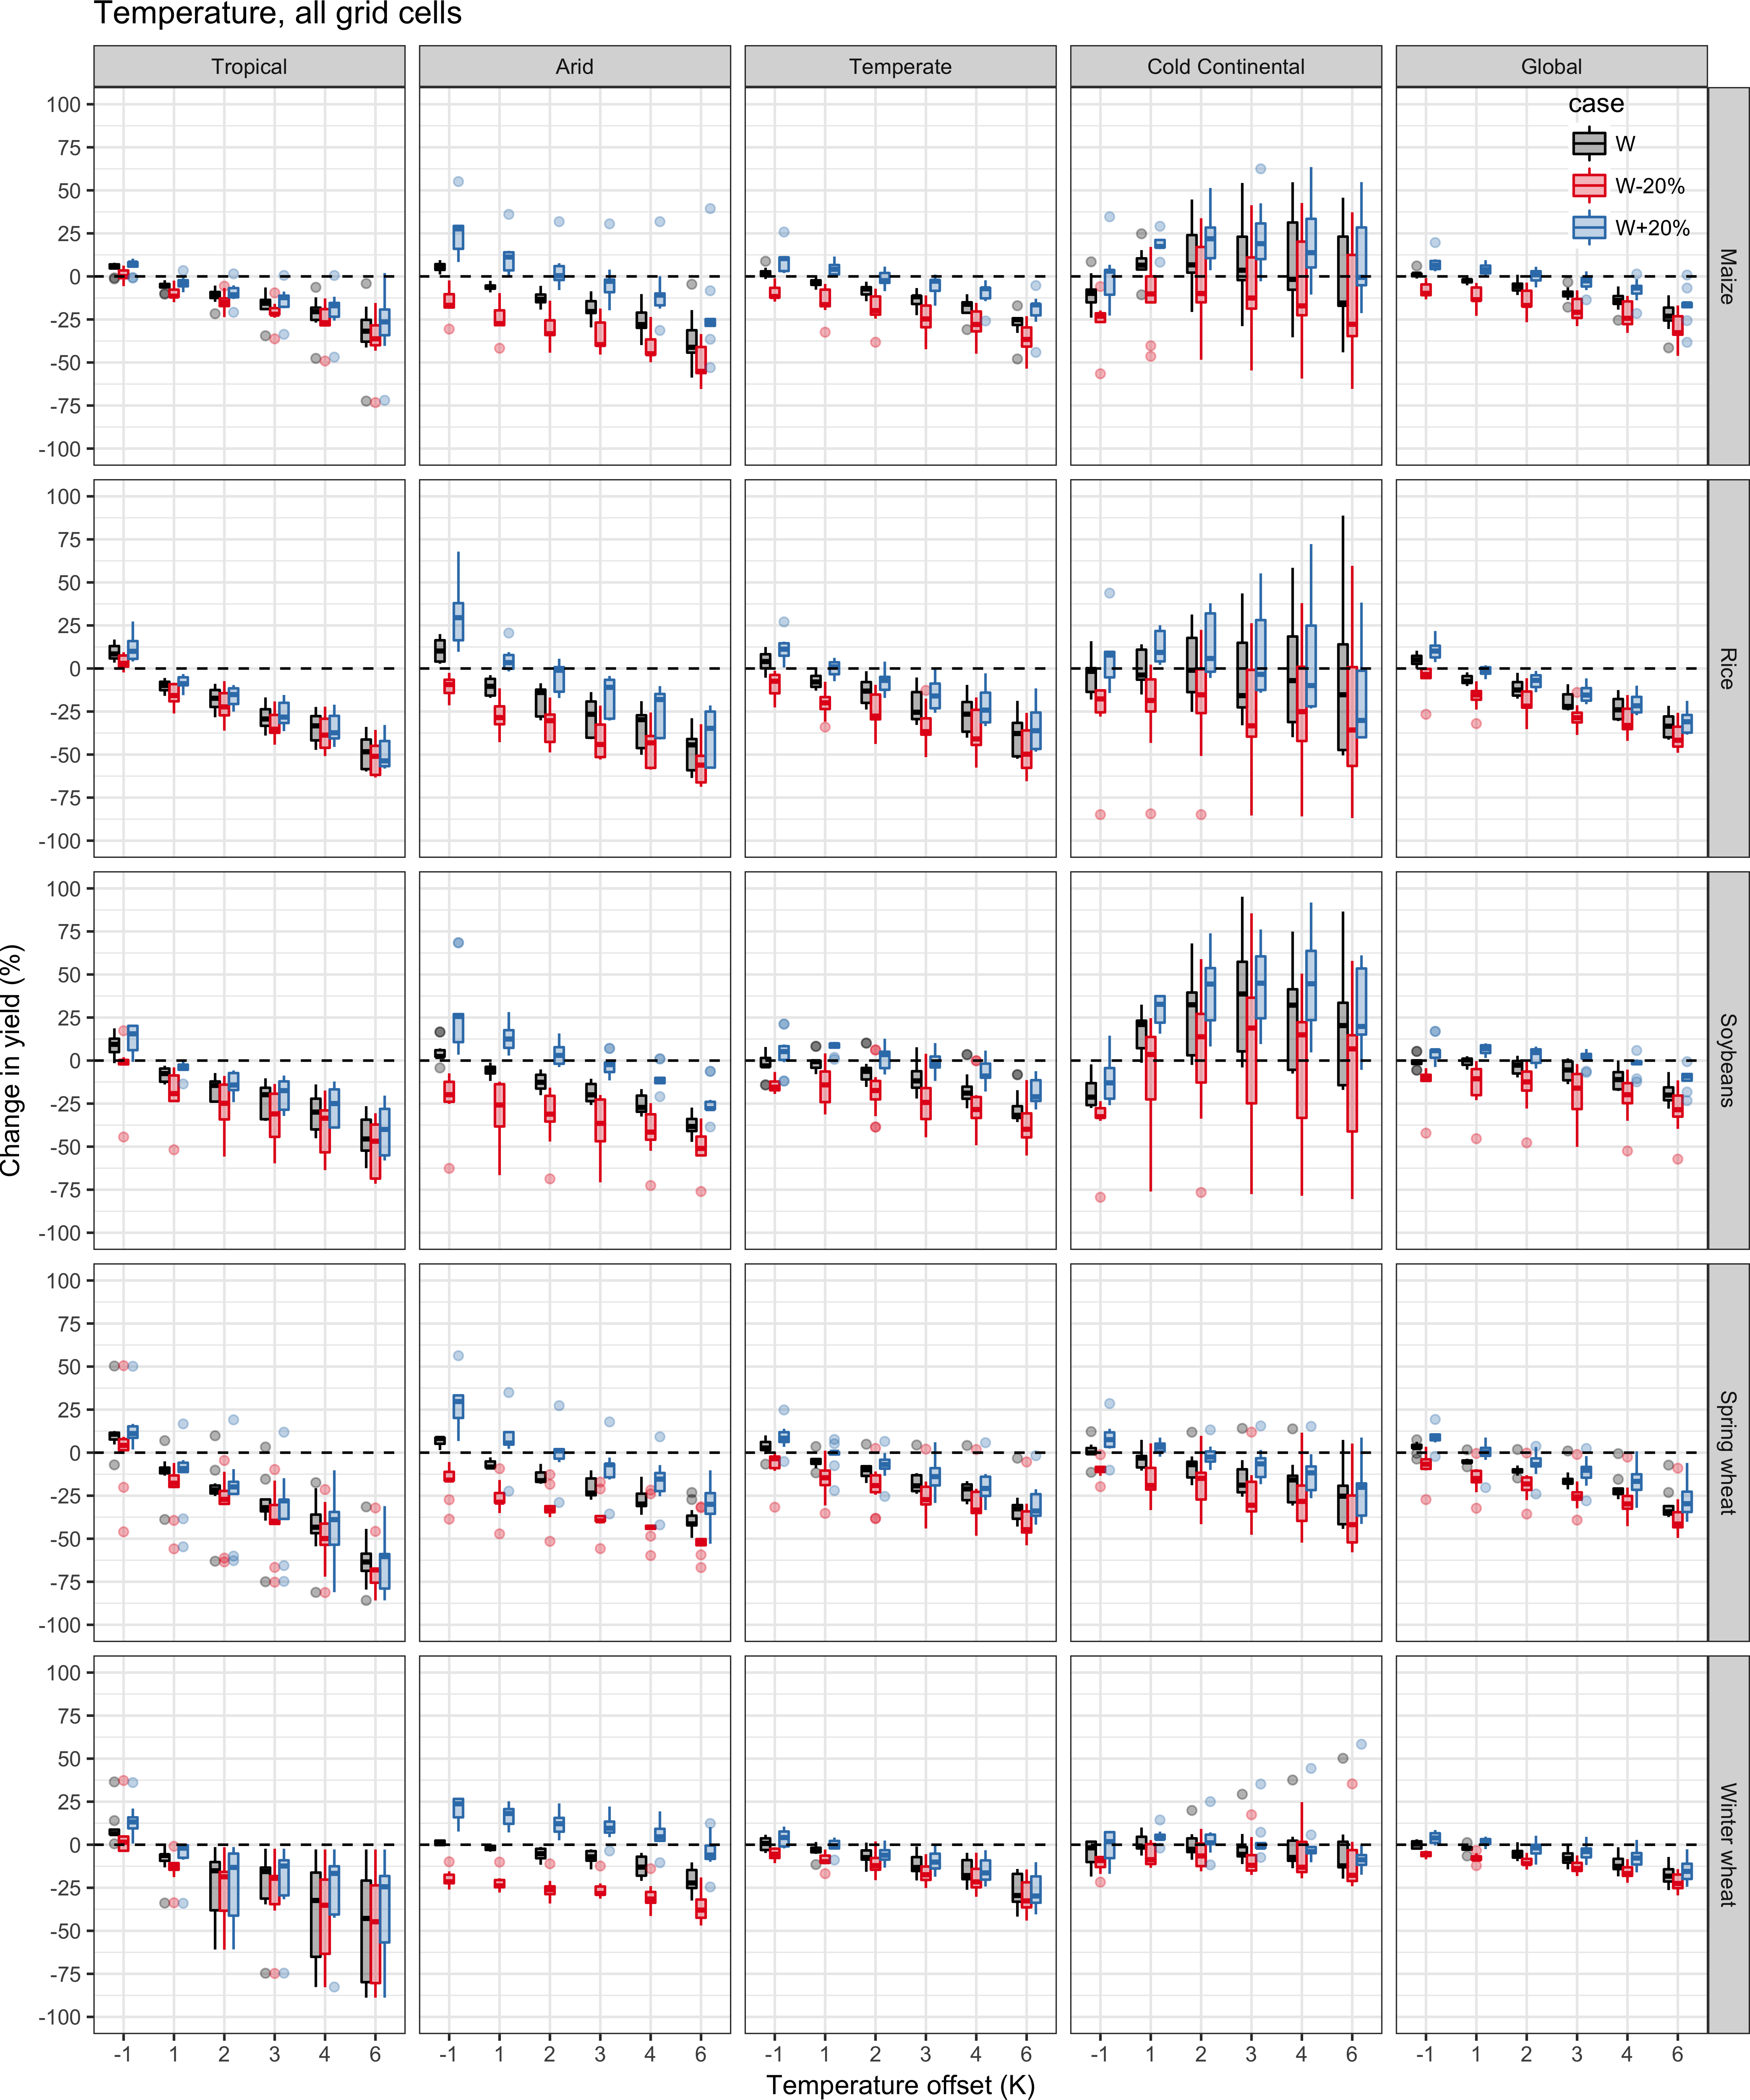
\includegraphics[width=\textwidth]{s_sim_CG_T.png}
\caption{Same as main Figure 5a for all crops.}
\label{fig:temperautre}
\end{figure}

\begin{figure}[h!]
\centering
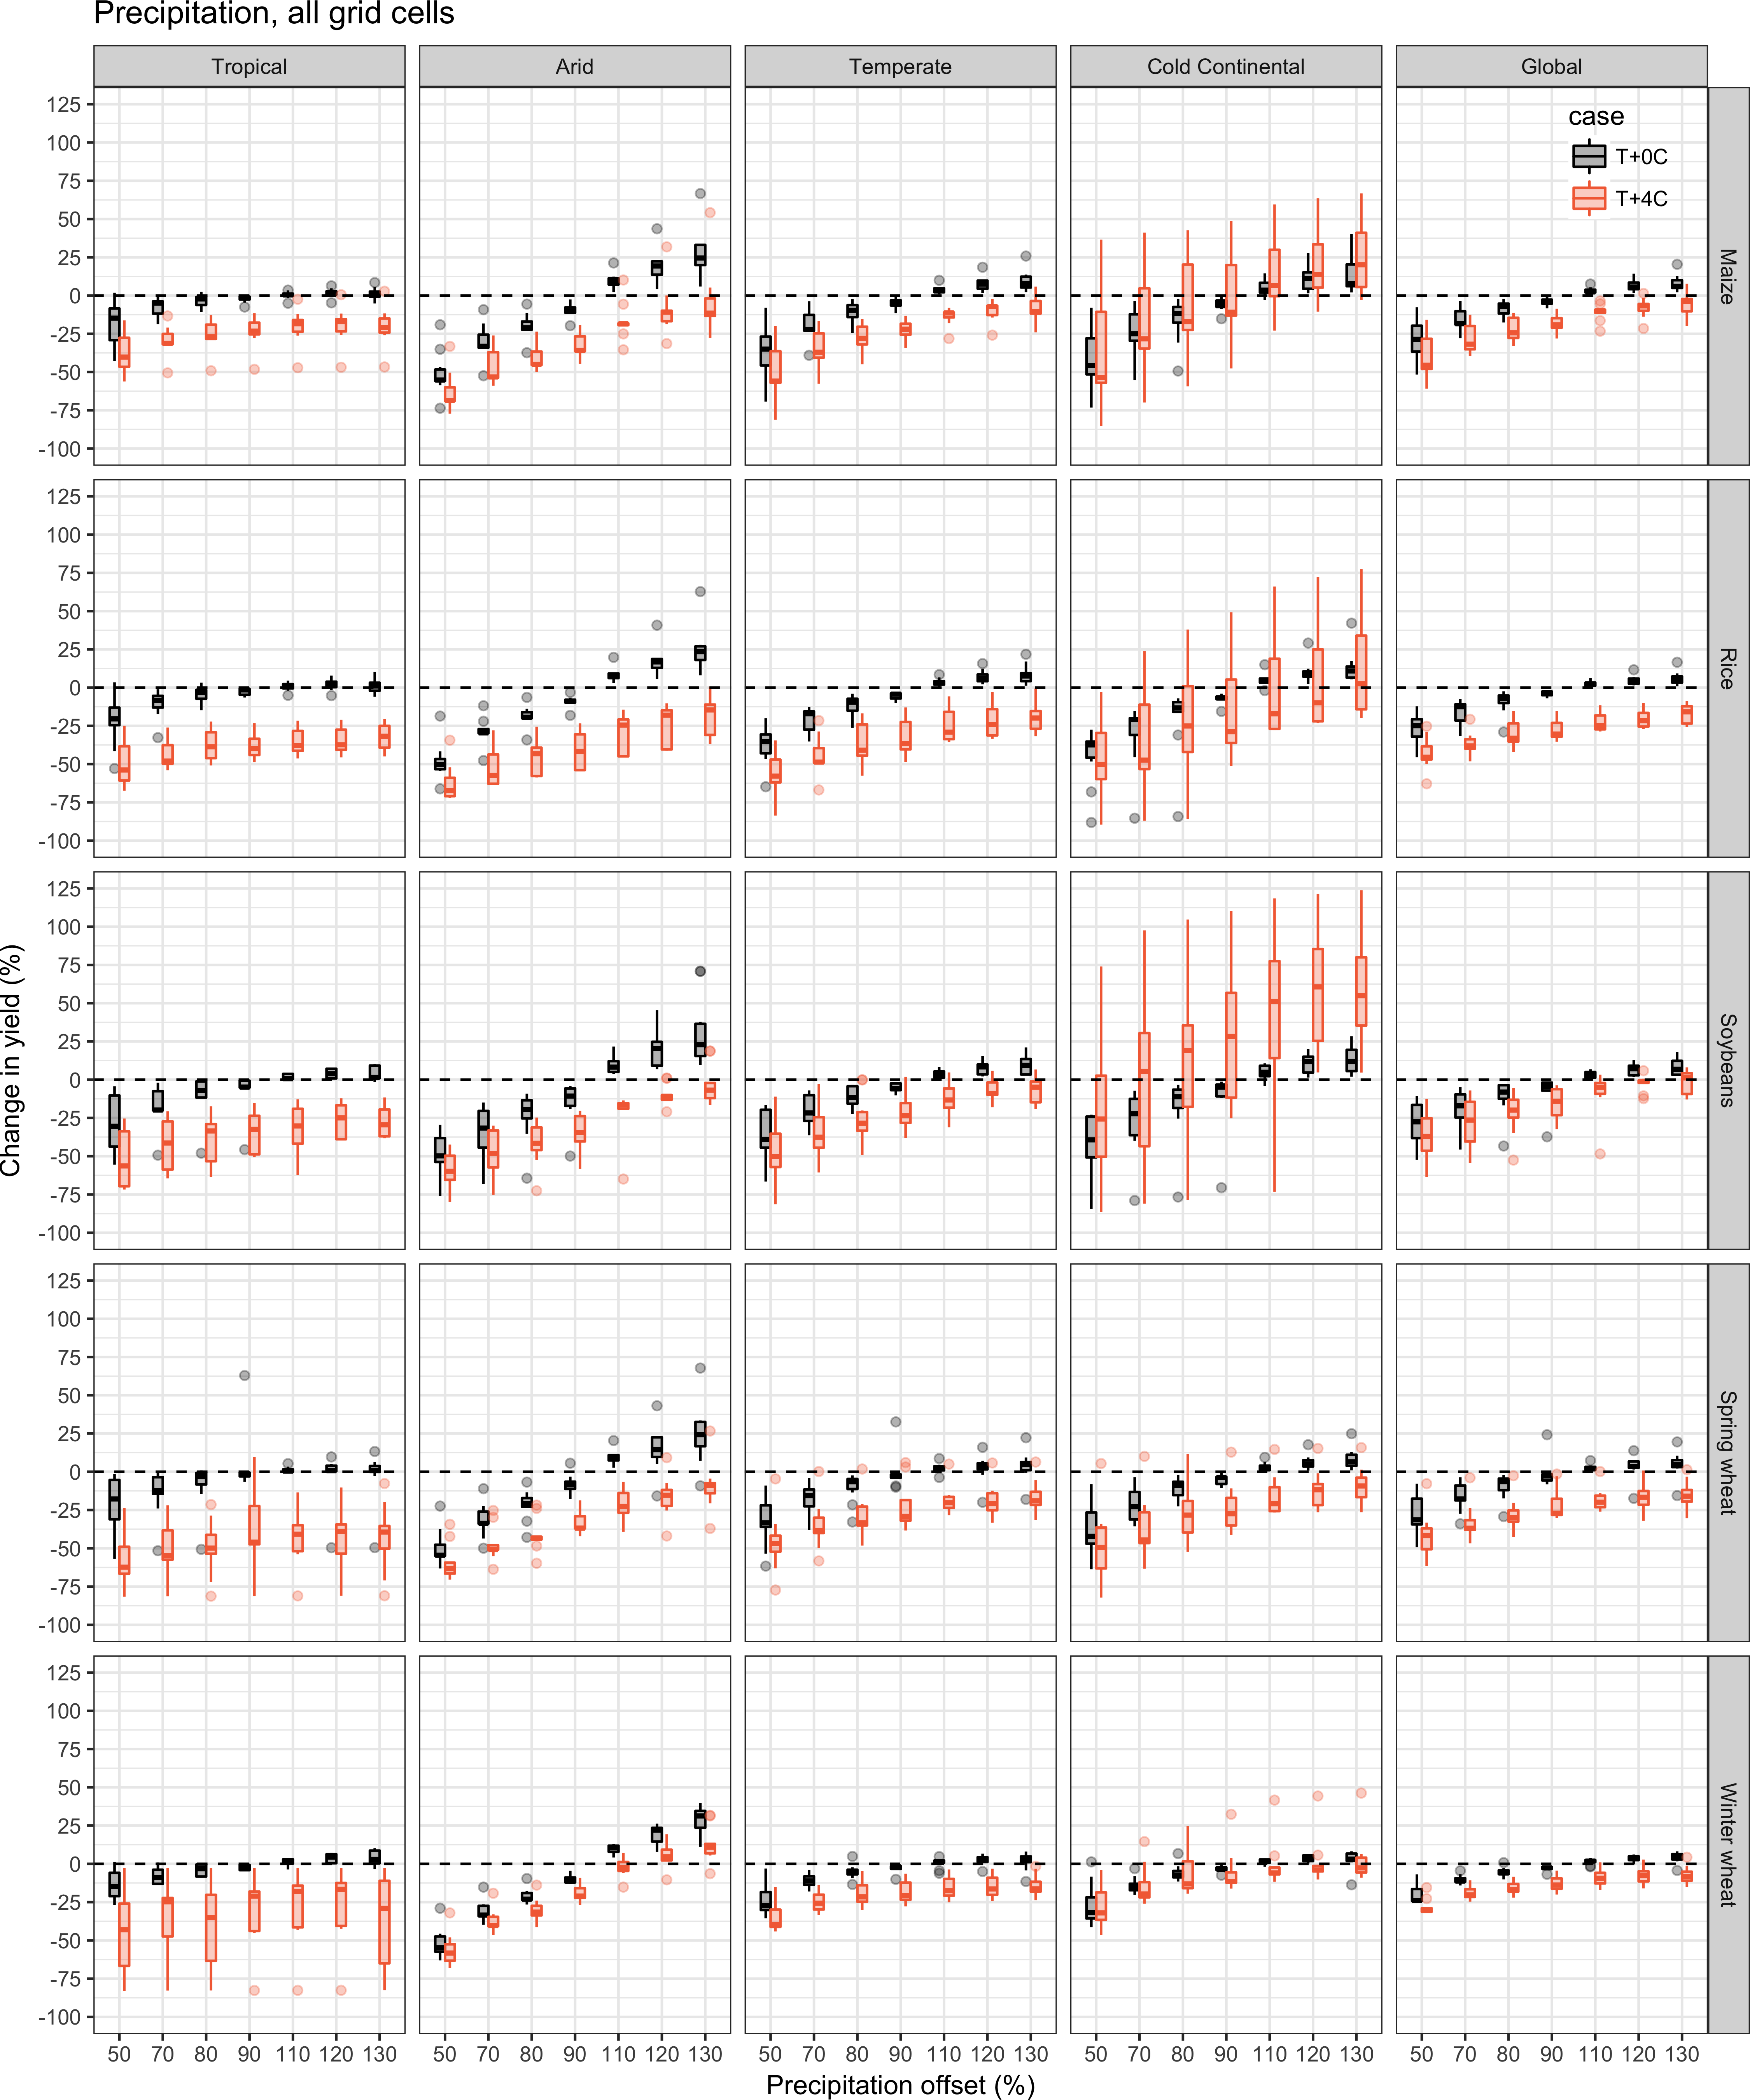
\includegraphics[width=\textwidth]{s_sim_CG_W.png}
\caption{Same as main Figure 5b for all crops.}
\label{fig:water}
\end{figure}

\begin{figure}[h!]
\centering
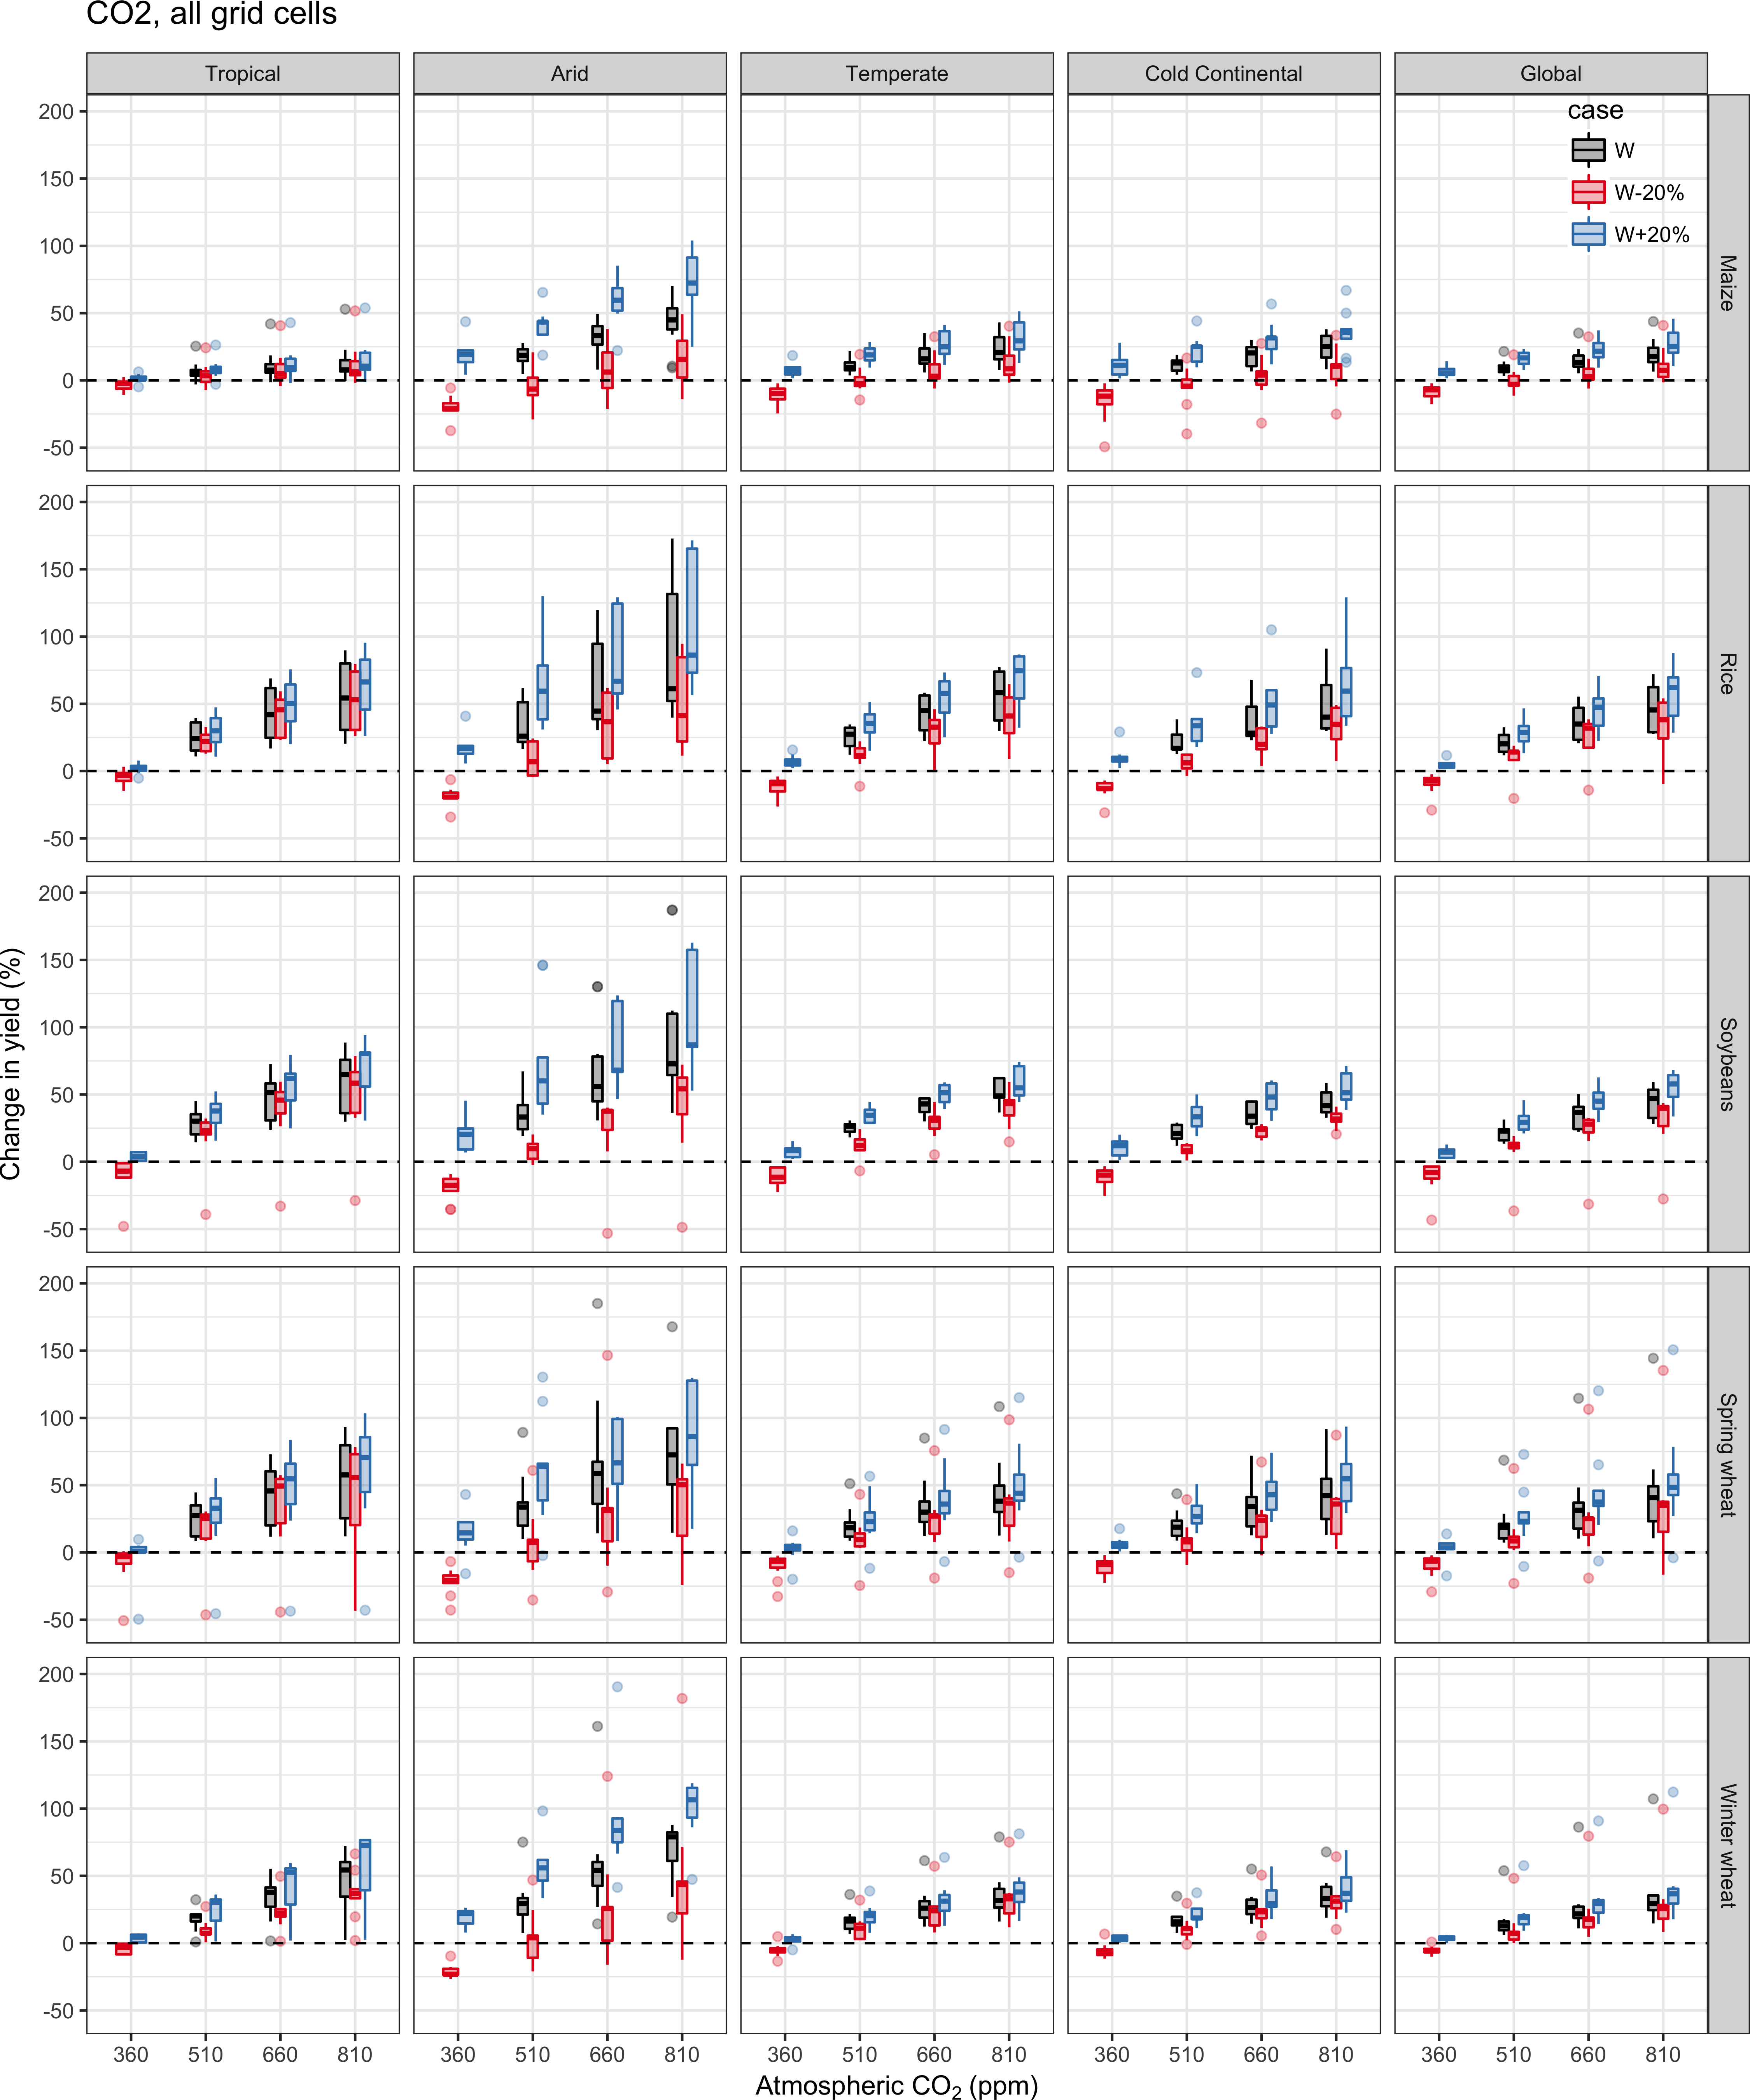
\includegraphics[width=\textwidth]{s_sim_CG_C.png}
\caption{Same as main Figure 6a for all crops.}
\label{fig:carbon}
\end{figure}

\begin{figure}[h!]
\centering
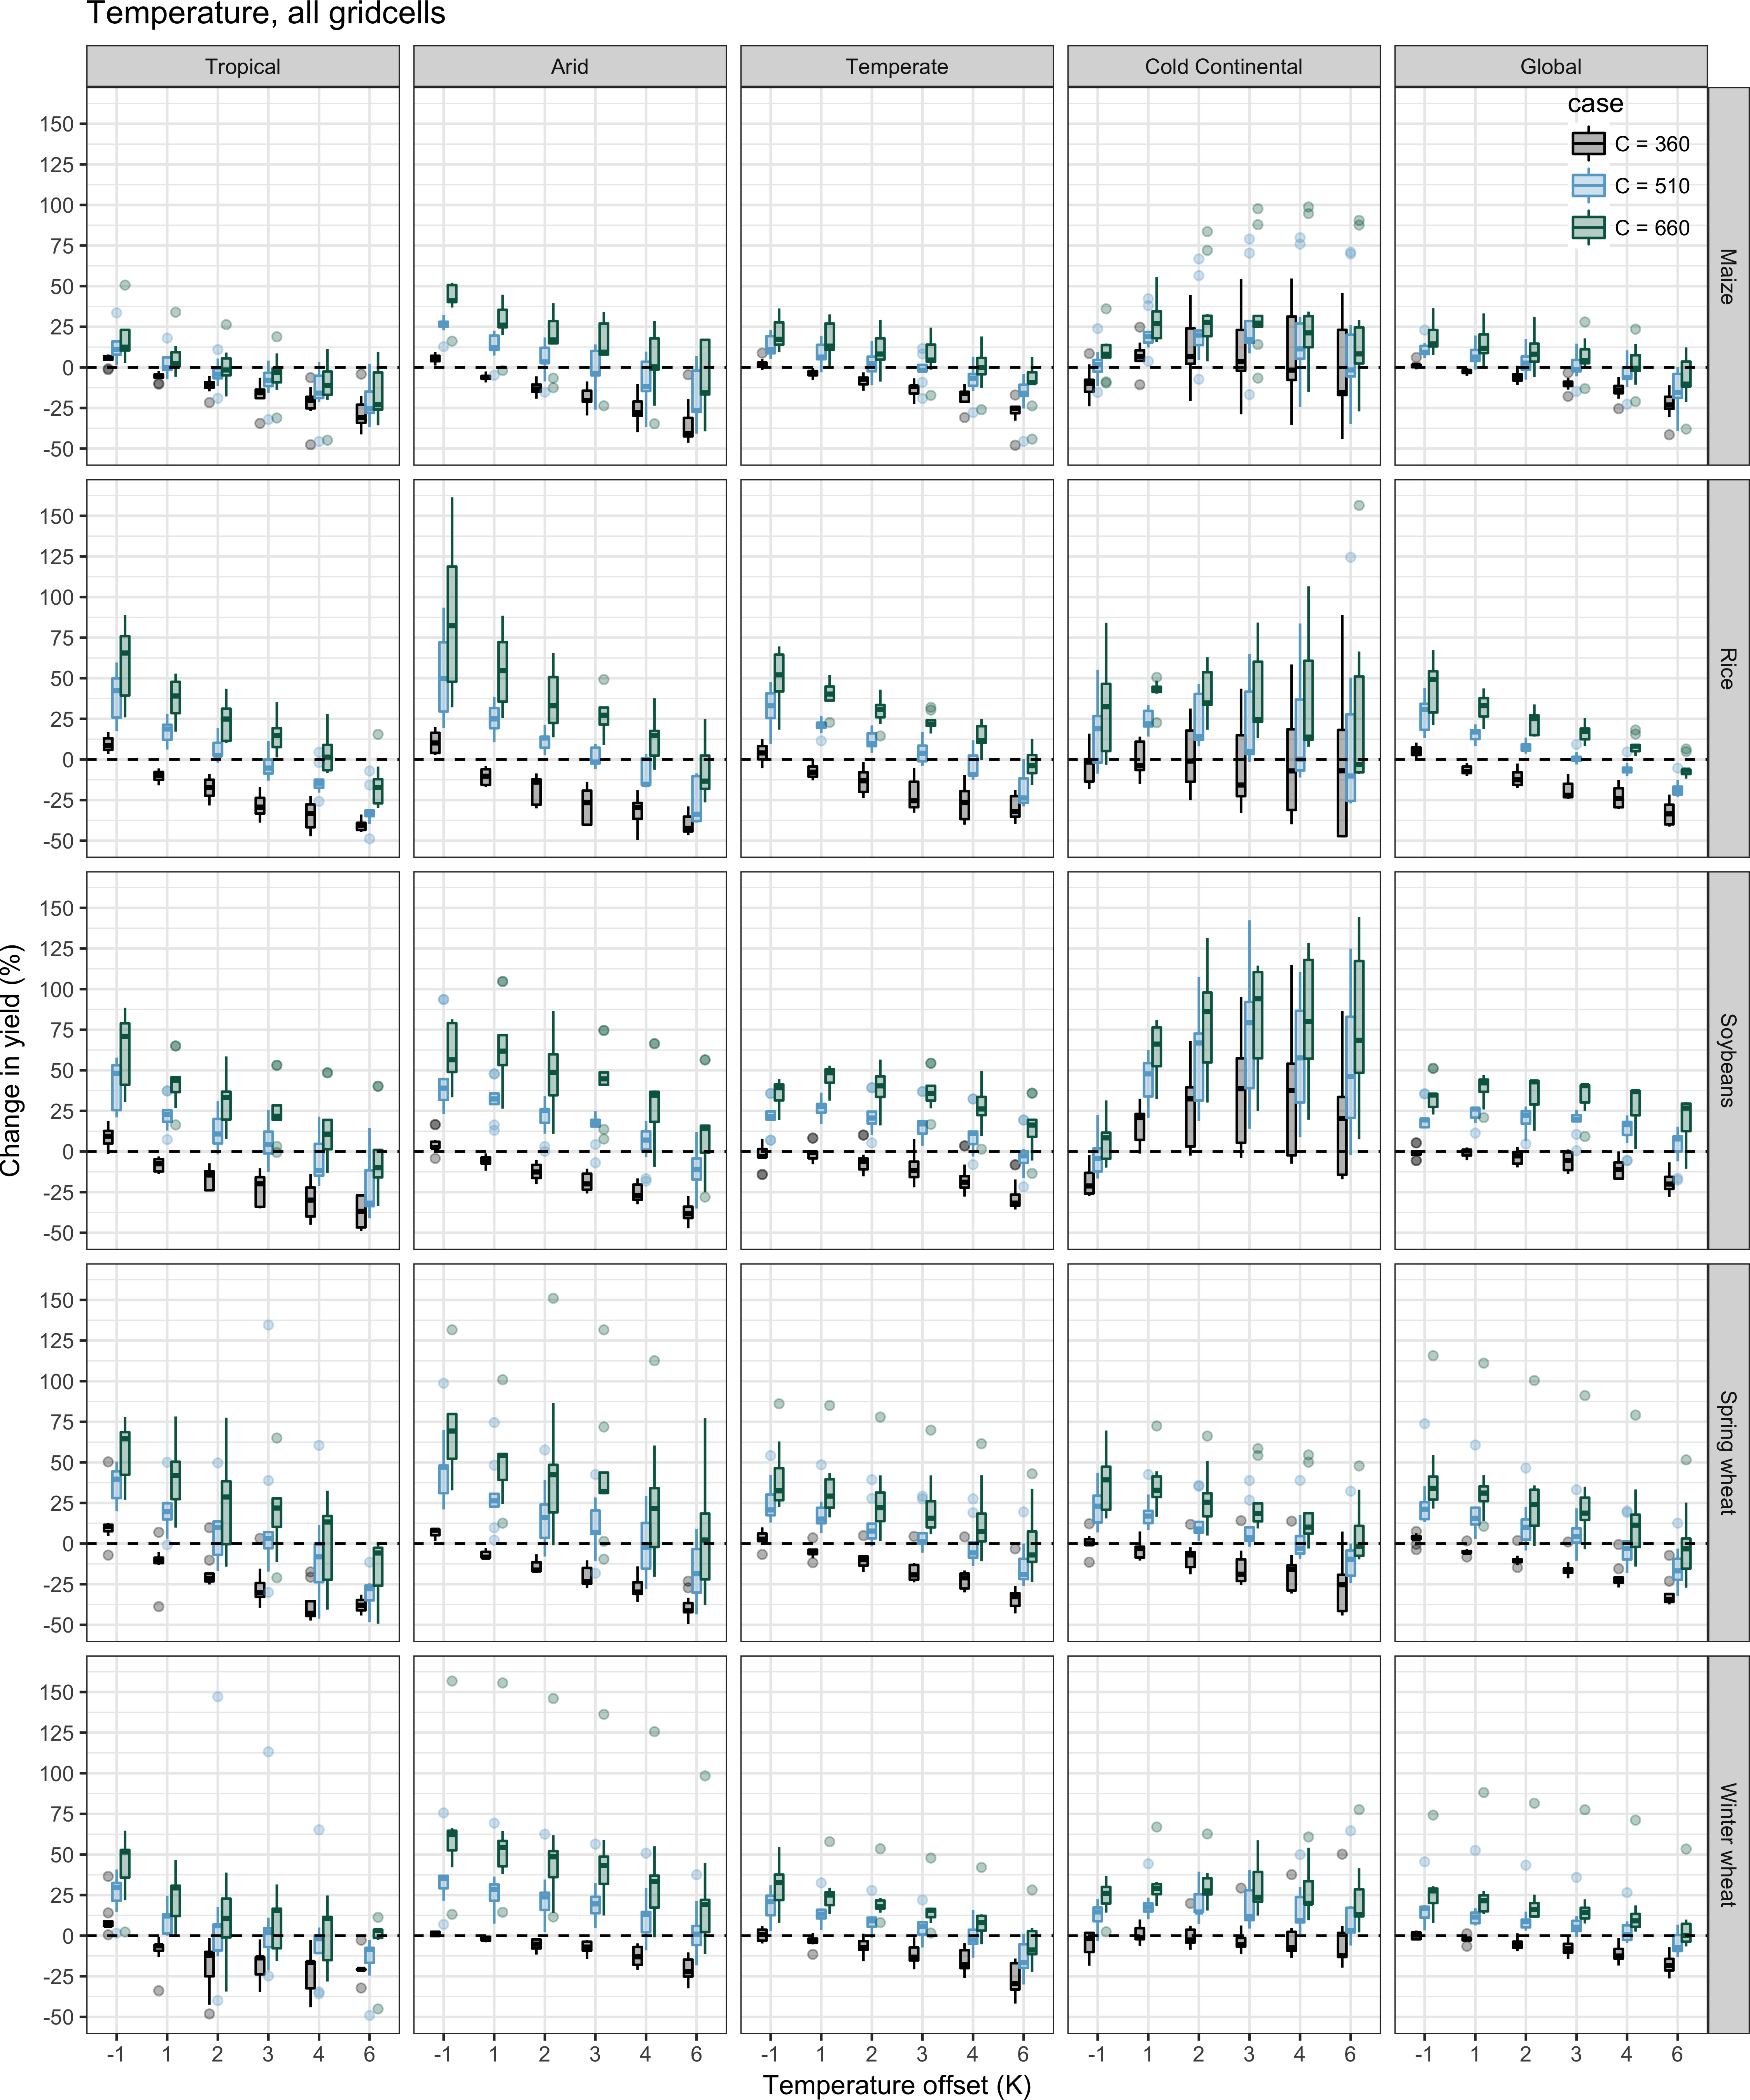
\includegraphics[width=\textwidth]{s_sim_CG_TC.png}
\caption{Same as main Figure 6b for all crops.}
\label{fig:carbontemp}
\end{figure}

\end{document}


